\section{Transformada inversa}

%\begin{frame}{Técnica de la Transformada Inversa}
%    \begin{itemize}
%        \item La técnica de la transformada inversa puede utilizarse para generar variables aleatorias con distribución exponencial, uniforme, Weibull y triangular \cite{BCN}. 
%        \item Adicionalmente es la principal técnica para generar muestras de distribuciones discretas así como de distribuciones empíricas \cite{BCN}
%        \item Es principio se puede utilizar para cualquier tipo de distribución, pero es más útil cuando la función de densidad acumulada $F(x)$ es de una forma tal que su función inversa $F^{-1}$ puede calcularse fácilmente.
%    \end{itemize}   
%\end{frame}

\begin{frame}{Método de la transformada inversa}
    \begin{itemize}
        \item Emplea el siguiente algoritmo:
    \begin{enumerate}
        \item Calcule la cdf $F(X)$ para la variable aleatoria $X$.
        \item Iguale $F(X)=U$ para el rango de $X$, siendo $U$ un número aleatorio.
        \item Resuelva la ecuación $F(X)=U$ para $X$ es términos de $U$, es decir, encuentra la función inversa $X=F^{-1} \left(U\right)$.
        \item Genere los números aleatorios $R_1, R_2, R_3, \dots$ y calcule el valor correspondiente en la distribución de la variable aleatoria como \begin{equation*}
            X=F^{-1} \left(R_i\right)
        \end{equation*}
    \end{enumerate}
    \end{itemize}
\end{frame}

\begin{frame}{Método de la transformada inversa}
    \begin{figure}
        \centering
        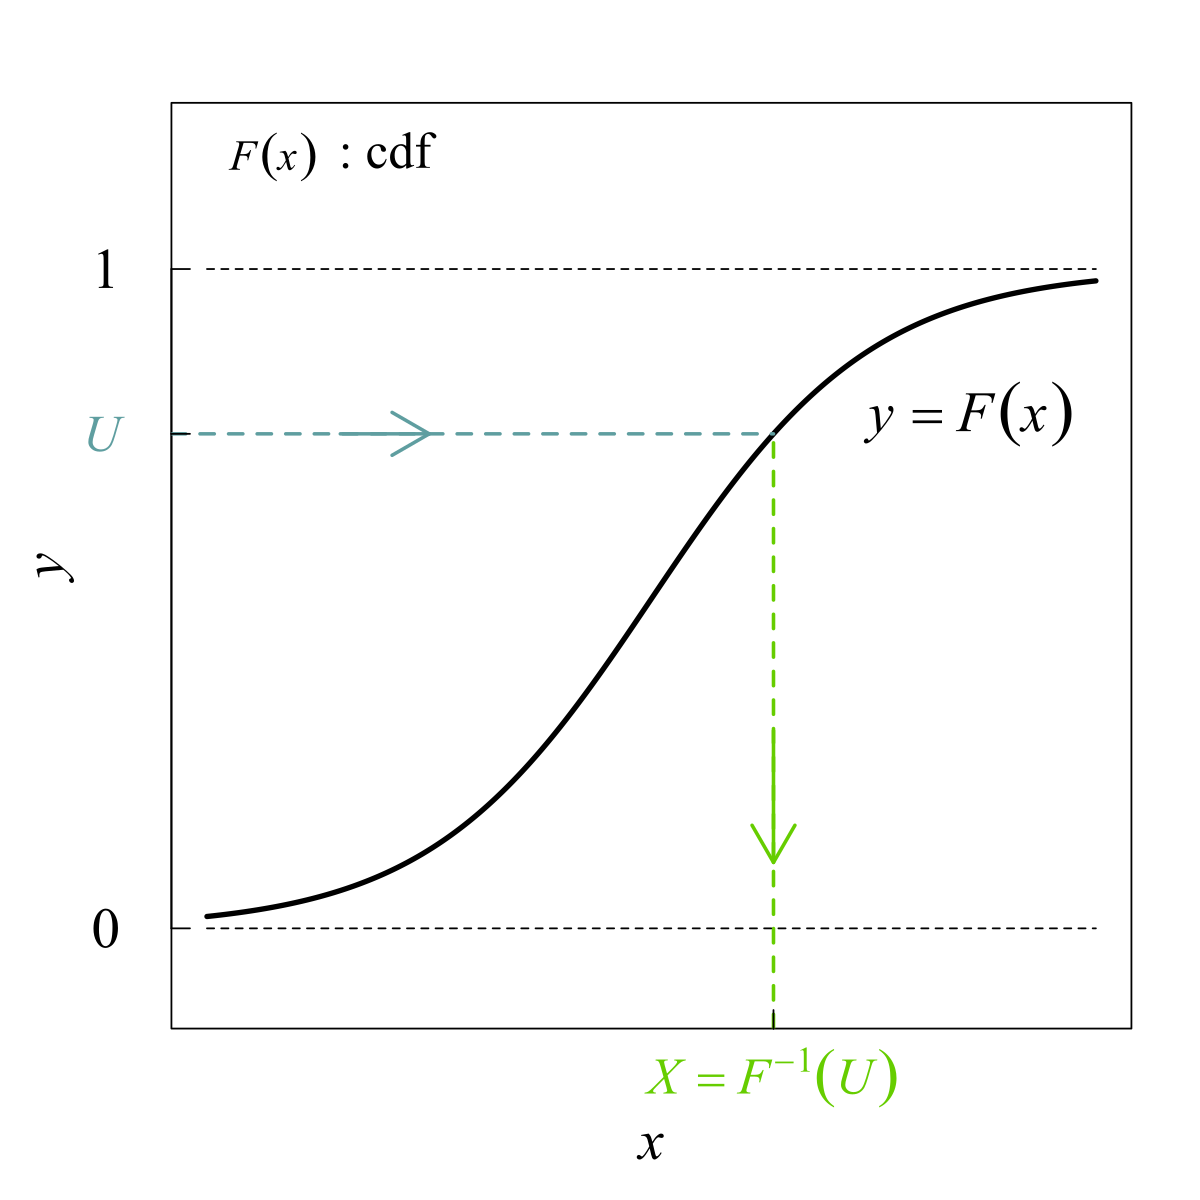
\includegraphics[width=6cm]{images/transf_inv.png}
        \caption{Método de la transformada inversa}
        \label{fig:my_label}
    \end{figure}    
\end{frame}

\begin{frame}{Método de la transformada inversa}{Distribución uniforme}
    \begin{itemize}
        \item La función de probabilidad acumulada de la distribución uniforme
        \begin{equation*}
            F(x)=\left\{\begin{array}{cc}
                 0 & x < a \\
                 \frac{x-a}{b-a} & a \leq x \leq b \\
                 1 & x > b
            \end{array}\right.
        \end{equation*}
        \item Aplicando la transformada inversa y despejando se tiene el generador \begin{equation*}
            X=(b-a)R+a
        \end{equation*}
    \end{itemize}
\end{frame}

\begin{frame}{Método de la transformada inversa}{Distribución exponencial}
    \begin{itemize}
        \item La función de probabilidad acumulada de la distribución exponencial
        \begin{equation*}
            F(x)=\left\{\begin{array}{cc}
                 1-e^{-\lambda x} & x \geq 0  \\
                 0 & x < 0
            \end{array}\right.
        \end{equation*}
        \item Al aplicar la transformada inversa y despejando se tiene el generador \begin{equation*}
            X=\frac{-\ln{(1-R)}}{\lambda}
        \end{equation*}
    \end{itemize}
\end{frame}

\begin{frame}{Método de la transformada inversa}{Distribución triangular}
    \begin{itemize}
        \item La función de probabilidad acumulada de la distribución triangular $\left[a,m,b\right]$ está dada por
        \begin{equation*}
            F(x)=\left\{\begin{array}{ll}
                 0 & x < a  \\
                 \frac{\left(x-a\right)^2}{\left(b-a\right)\left(m-a\right)} & a\leq x\leq m \\ 
                 1-\frac{\left(b-x\right)^2}{\left(b-a\right)\left(b-m\right)} & m\leq x\leq b \\ 
                 1 & b<x
            \end{array}\right.
        \end{equation*}
    \end{itemize}
\end{frame}

\begin{frame}{Método de la transformada inversa}{Distribución triangular}
    \begin{itemize}
        \item Note que si $X \sim TRIA\left(0,\frac{m-a}{b-a},1\right)$, entonces \begin{equation*}
            X'=a+(b-a)X \sim TRIA\left(a,m,b\right) 
        \end{equation*}
        \item El generador para $X$ se puede obtener a partir de la transformada inversa como
        \begin{equation*}
            X=\left\{\begin{array}{ll}
            \sqrt{m'R} & 0 \leq R \leq m'\\
            1-\sqrt{\left(1-m'\right)\left(1-R\right)} & m'<R\leq 1
            \end{array}\right.
        \end{equation*}
        donde $m'=\frac{m-a}{b-a}$
    \end{itemize}
\end{frame}

\begin{frame}{Método de la transformada inversa}{Distribuciones discretas}
    \begin{itemize}
        \item Suponga que se quiere generar una variable aleatoria discreta con función de probabilidad de masa:
    \begin{equation*}
        P\left\{X=x_j\right\}=p_j, ~ j=0,1,\dots , ~\sum_j{p_j}=1
    \end{equation*}
    \item El algoritmo a emplear es:
    \begin{enumerate}
        \item Genere un número aleatorio $R$
        \item Si $R<p_0$ entonces $X=x_0$ y pare
        \item Si $R<p_0+p_1$ entonces $X=x_1$ y pare
        \item Si $R<p_0+p_1+p_2$ entonces $X=x_2$ y pare
        \item $\vdots$
    \end{enumerate}
    \end{itemize}
\end{frame}